Hubo2 Plus, Hubo for short, is a 130 $cm$ (4' 3'') tall, 42 $kg$ (93 $lb$) full-size humanoid robot.  
It was designed and constructed by Prof Jun-Ho Oh and the Hubo Lab at the Korean Advanced Institute of Science and Technology\cite{hubo-first}.
Hubo has 2 arms, 2 legs and a head, making it anthropomorphic to a human.  
It boasts 38 degrees of freedom (DOF) consisting of 6x in each leg, 6x in each arm, 5x in each hand, 3x in the neck, and 1x in the waist.
All joints with the exception of the fingers are high gain PD position controlled.
The fingers are PWM controlled.
It has a three axis force torque (FT) sensor on leg between the end of the ankle and the foot and on the arm where it connects to the hand.
Additionally it has accelerometers on each foot and a six axis inertial measurement unit (IMU) slightly below it's weight (approximately the centre of mass).
The reference commands for all of the joints are sent from the primary control computer (x86) to the individual motor controllers via two Controller Area Network (CAN) buses.
There are currently eight Hubo's functioning in the United States as of December 2012.
Four reside at Drexel University and one at Georgia Tech, Perdue, Ohio State and MIT.
Jaemi Hubo is the oldest of the Hubos in America and has been at the Drexel Autonomous Systems Lab\footnote{Drexel Autonomous Systems Lab: http://dasl.mem.drexel.edu/} (DASL) since 2008\cite{jaemiHuboSRM}.
Fig.~\ref{fig:hubo} shows the major dimensions of Hubo.

\begin{figure}[thpb]
  \centering
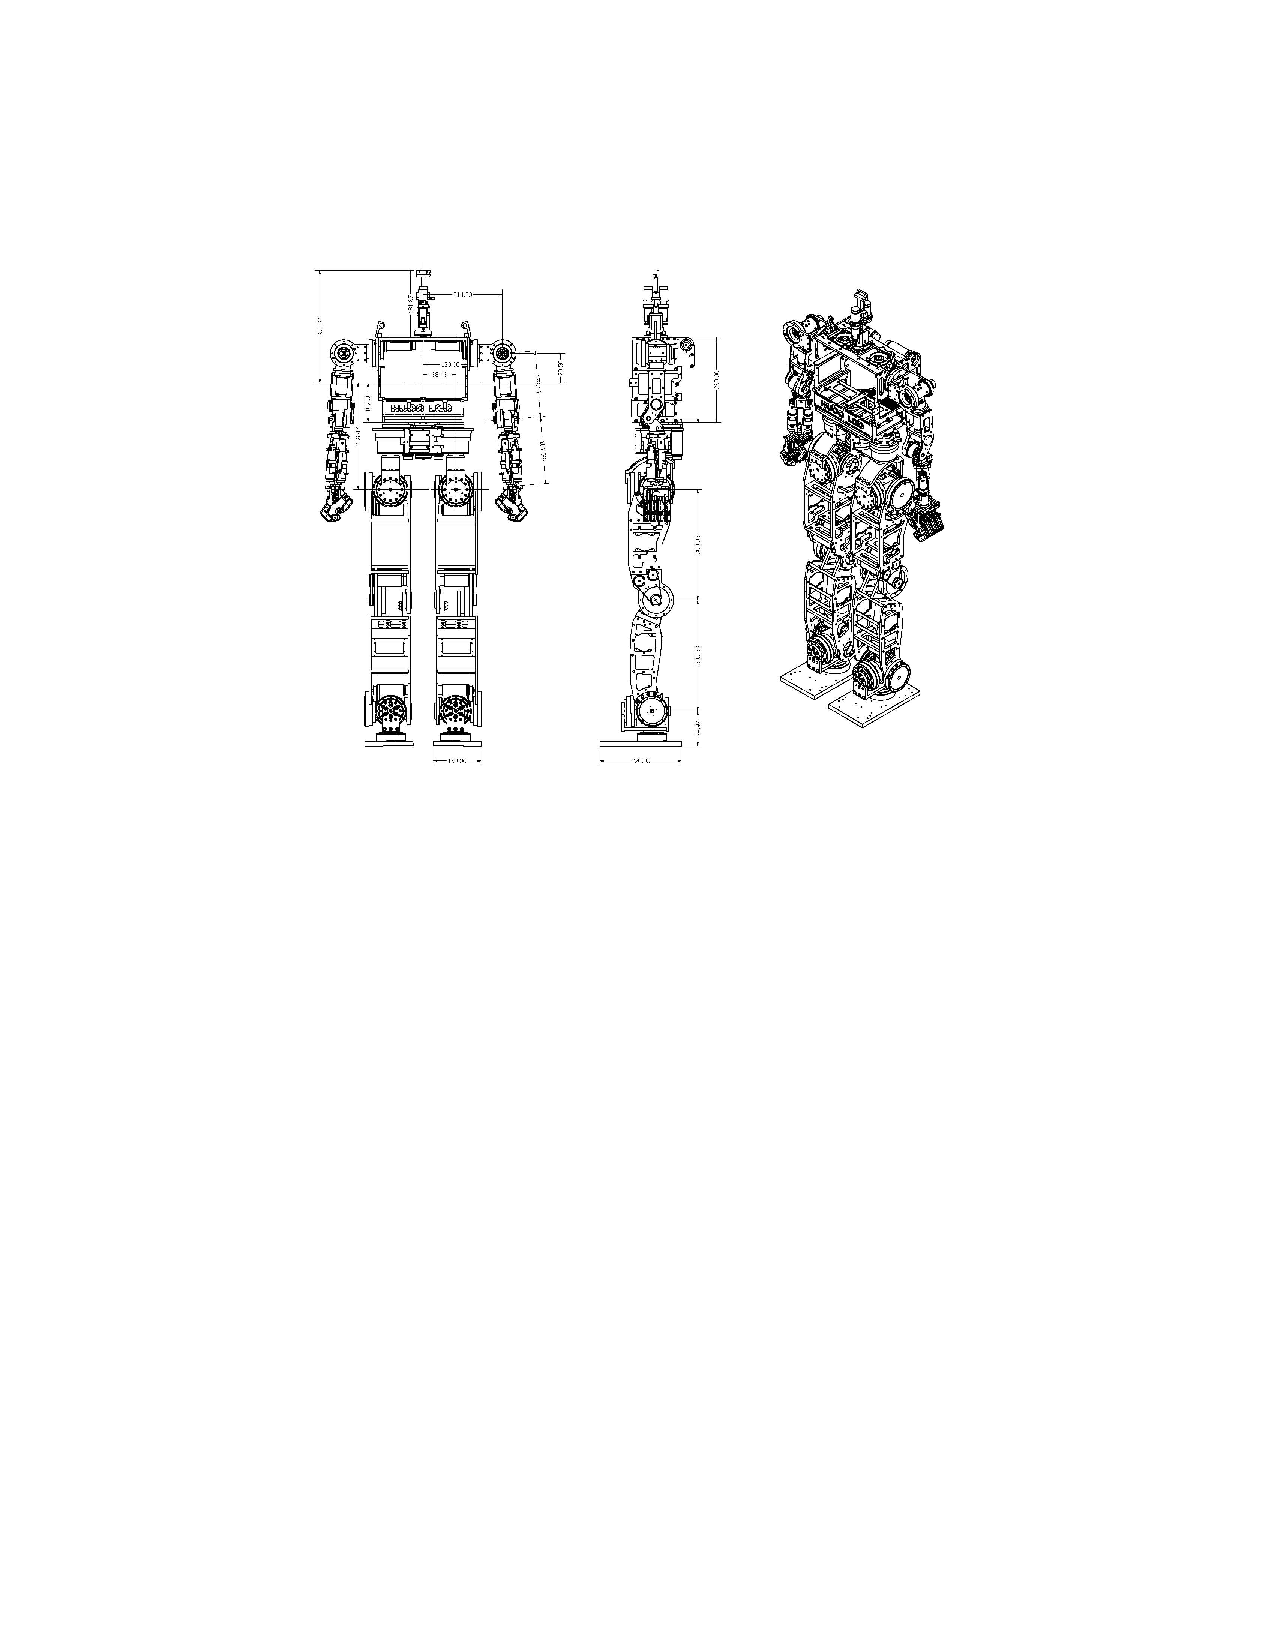
\includegraphics[width=1.0\columnwidth]{./pix/huboSkel.pdf}
  \caption{Hubo2 platform: 130 $cm$ tall full-size humanoid robot weighing 37 $kg$.  It has 38 DOF consisting of 6x in each leg, 6x in each arm, 5x in each hand, 1x in the waist, and 3x in the neck.}
  \label{fig:hubo}
\end{figure}

Hubo now runs on the Linux based, open-source, BSD licensed, system called Hubo-Ach.  
The overarching goal of the Hubo-Ach system is to create an easy to use interface between the Hubo hardware and the software environment.  
All system design decisions are made with the users, programmers and developers of the Hubo in mind.
This design philosophy streamlines closed-loop controller implementation, human robot interaction development and the utilization of popular robot related systems such as ROS\footnote{ROS: http://www.ros.org/} (Robot Operating System), OpenRAVE\footnote{OpenRAVE: http://openrave.org/} and MATLAB\footnote{MATLAB: http://www.mathworks.com/} on the Hubo platform.
Hubo-Ach also needs to be inherently robust because it is one of the software platforms being used by the DRC-Hubo\footnote{DRC-Hubo: http://drc-hubo.com/} DARPA Robot Challenge\footnote{DARPA Robot Challenge: http://www.theroboticschallenge.org/} team where DASL is leading over half a dozen university labs.

Thus Hubo-Ach has great advantages over the Windows based software traditionally run on Hubo.
Hubo is traditionally run on software based in Windows utilizing the Real-Time framework called Real-Time Extensions (RTX) for Windows.
This software includes walking and other canned gestures with a user-friendly GUI making it a good choice for public demonstrations.
The overall system design is not conducive to adding additional closed-loop controllers, additional functionality or integration with third-party tools thus creating a critical-gap that must be crossed for increased software and controller development.
Hubo-Ach fills this critical-gap.


Hubo-Ach is the brain child of Daniel M. Lofaro\footnote{Daniel M. Lofaro: http://danlofaro.com/} of DASL at Drexel University in collaboration with \textit{Golems - The Humanoid Robotics Laboratory}\footnote{Golems - The Humanoid Robotics Labatory: www.golems.org/} at the Georgia Institute of Technology.  
The structure of Hubo-Ach can be seen in Fig.~\ref{fig:graph}.
Hubo-Ach is a single process that takes reference commands from independent processes and makes the current state of the robot available to those processes.
Hubo-Ach runs in the background taking care of all CAN communications between the sensors/motor and the Hubo-Ach system.
Each of the Hubo's motor controllers uses a phase lock loop (PLL) to lock onto the reference update rate $f_r$ and perform linear interpolation between each reference command.  
The resulting motor controller command frequency $f_m$ is equal to five times $f_r$.
This reduces the jerk applied to each joint.
In order for the PLL to work effectively Hubo-Ach must sets the references for each joint at the real-time rate of $f_r$.
The sensors data is also received at the real-time rate of $f_r$.
Hubo-Ach is currently run at a $f_r$ of 200 $Hz$ utilizing approximately 78\% of the bandwidth on the CAN bus.
All reference data is set by the independent processes using $SI$ units.
State data is made available to the independent processes in $SI$ units.


\begin{figure}[thpb]
  \centering
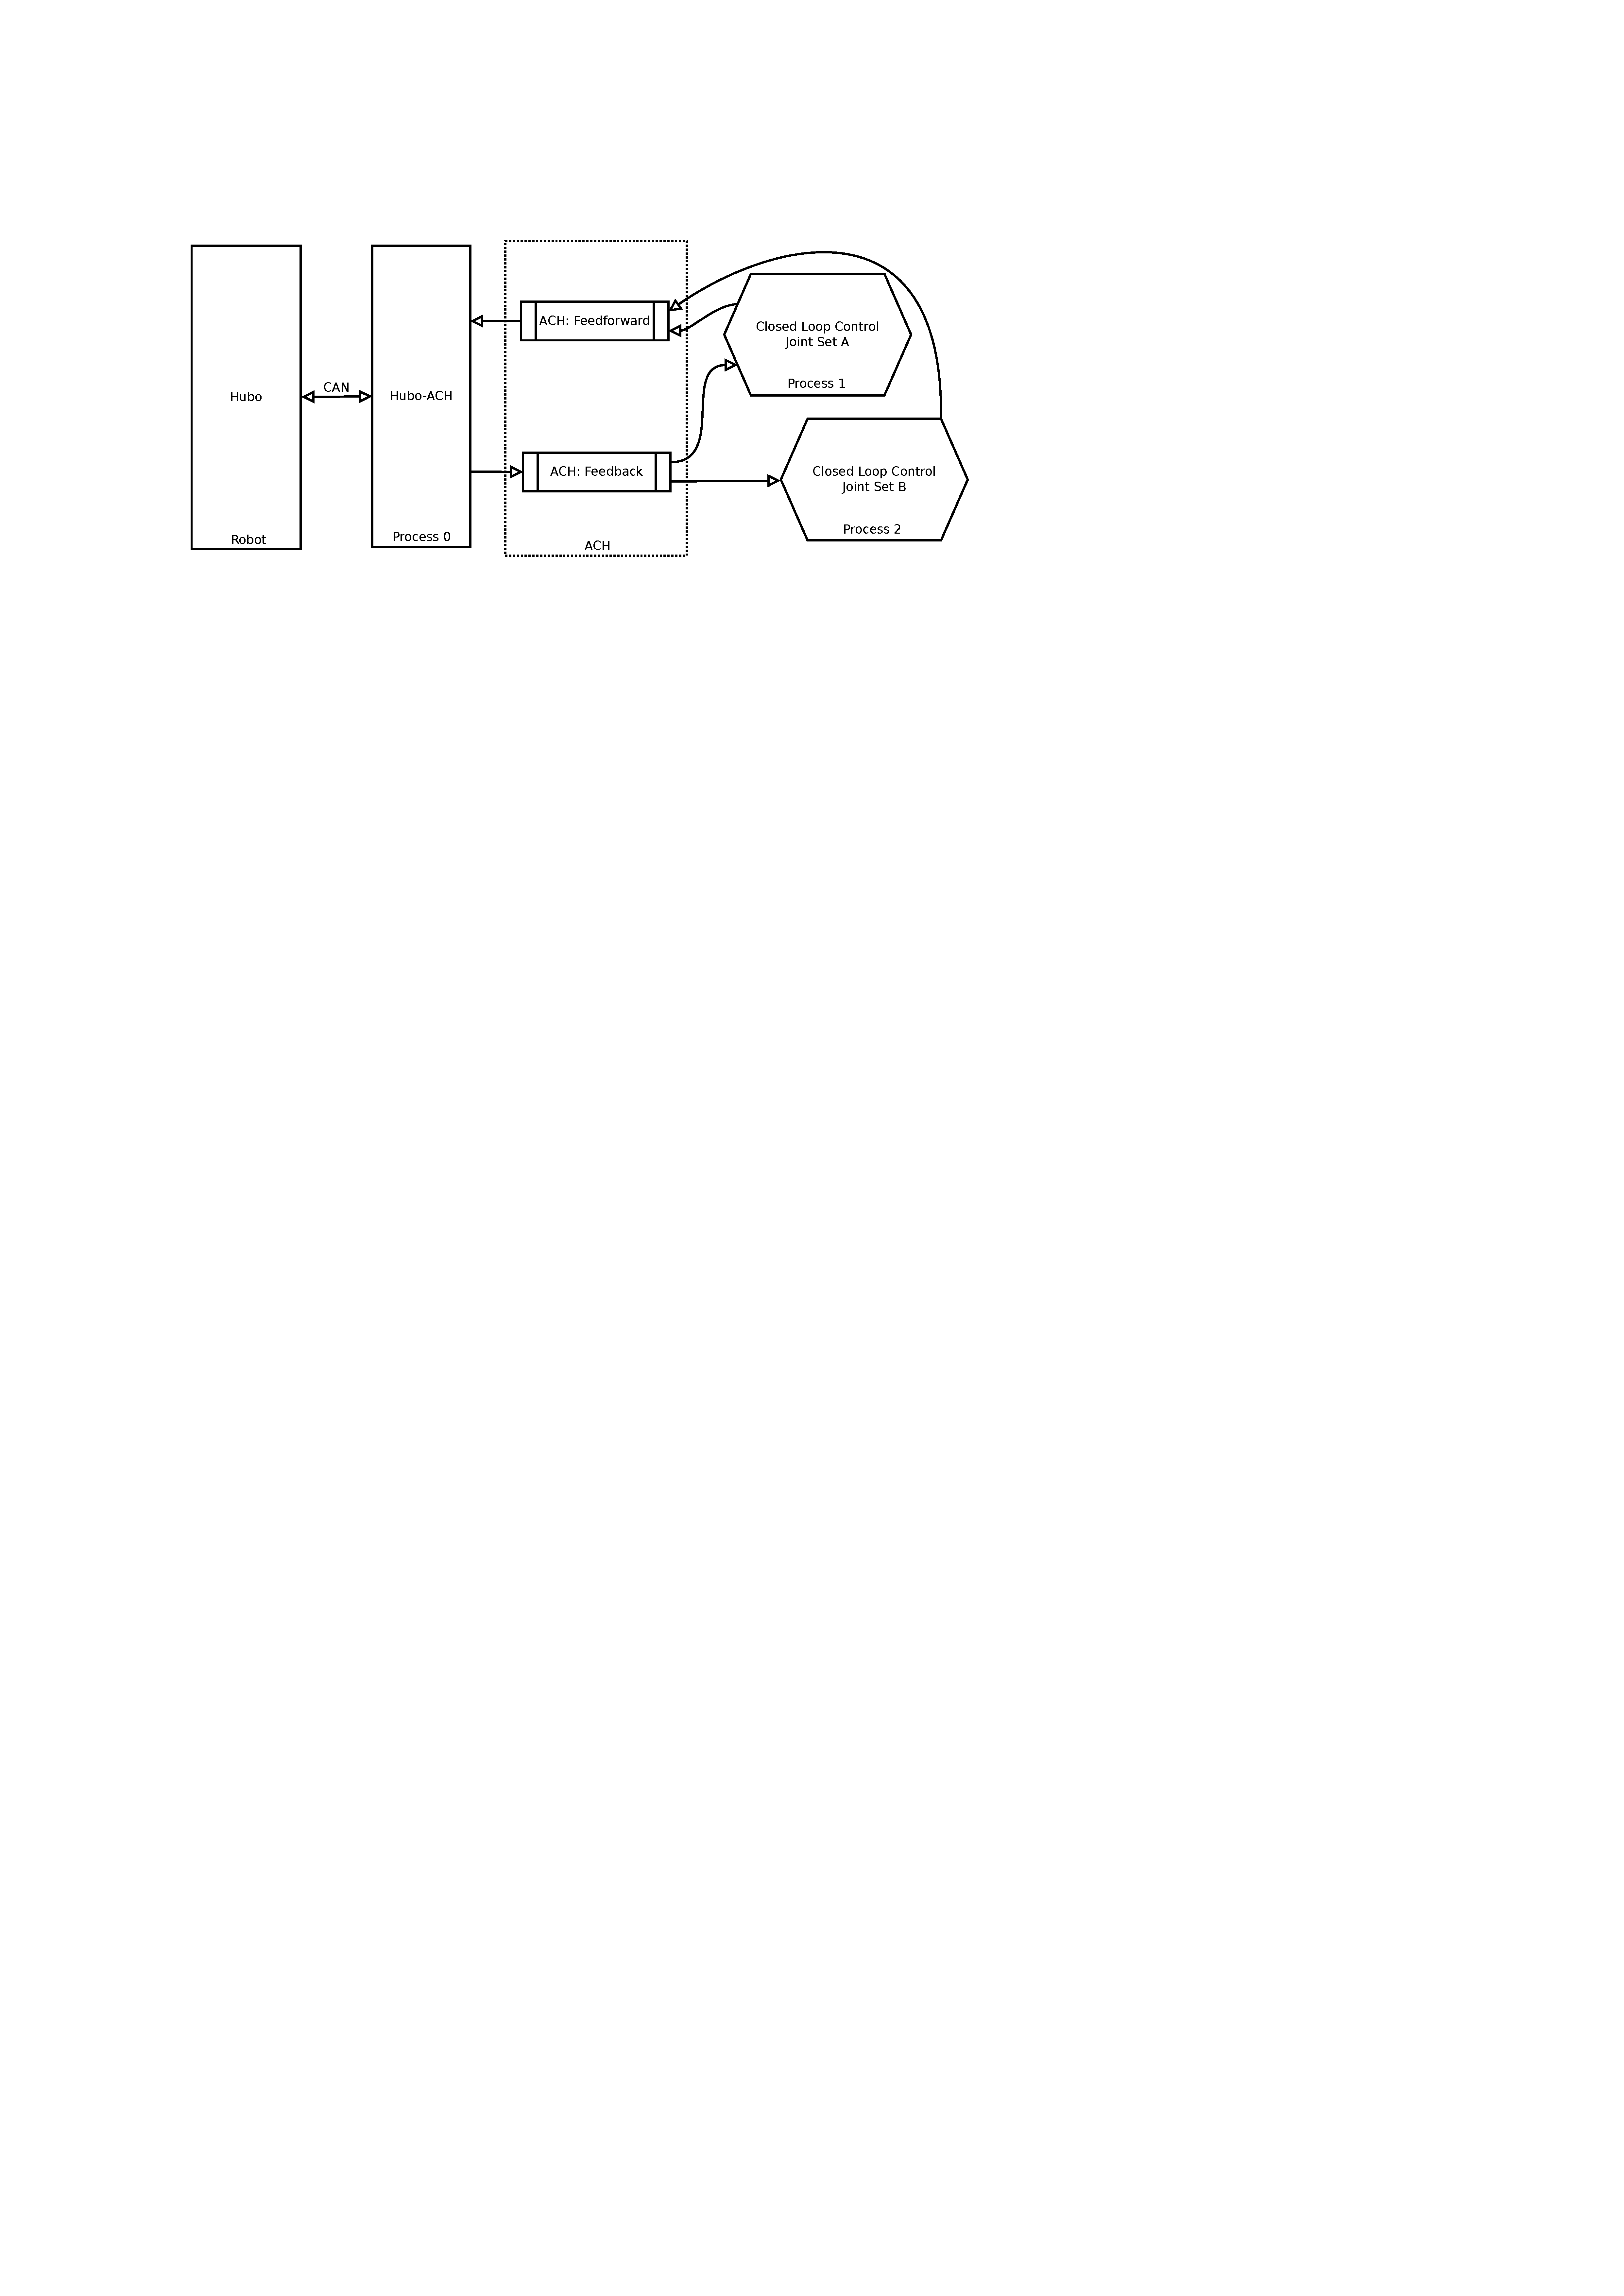
\includegraphics[width=1.0\columnwidth]{./pix/hubo-ach-diagram.pdf}
  \caption{Hubo Primary Controller (HPC) and system framework}
  \label{fig:graph}
\end{figure}


Controllers are run in separate processes from Hubo-Ach.
They communicate with Hubo-Ach via the Ach IPC.
Two Ach channels are made available; feed-forward: where the reference for each joint is set, and feed-back: where the state data is read.
Each controller can update the reference at any time, in real-time or not.
At the rising edge of the Hubo-Ach's real-time loop the most recent reference commands are the ones that are set to the Hubo.
This eliminates fear of the user over-utilizing the CAN bus and creating lag in the system.

The key point is that Hubo-Ach runs at a rate of $f_r$, commanding the motors with the references from the feed-forward channel no matter what rate the external controller is updating the feed-forward channel.  
Ach was chosen for the IPC because it makes the most recent data available first which is a requirement for this real-time application.

The DRC-Hubo team for the DARPA Robot Challenge consists of over half a dozen development teams spanning across several universities and utilizing multiple Hubo robots.  
This requires the ability to combine different controllers for different joints as well as communicate with ubiquitous robot tools such as OpenRAVE and MATLAB across multiple computers.
Because of the multi-process approach to Hubo-Ach, if one controller or piece of software that communicates with Hubo-Ach crashes the system does not totally fail. 
It only loses the functionality of the process that crashed.
This gives us the ability to combine software that is still in development without fear of crashing the robot.
This is not possible with the old single process multi-thread system.
Thus Hubo-Ach's inherent ability to safely deal with controller crashes becomes one of its most important features.





\begin{figure}[thpb]
  \centering
%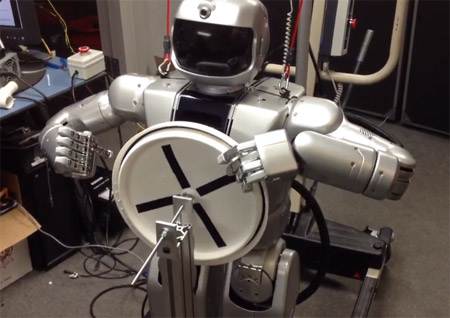
\includegraphics[width=1.0\columnwidth]{./pix/hubo_valve.png}
\includegraphics[width=1.0\columnwidth]{./pix/IMG_7628.JPG}
  \caption{Hubo running PHC turning a valve using trajectories created using Bi-RRTs. }
  \label{fig:valve}
\end{figure}

Current capabilities of the PHC system includes:

\begin{itemize}
\item Full Hubo2 Plus compatibility 
\item ROS support
\item Independent process for controllers
\item OpenRAVE trajectory playback
\item OpenHUBO integration 
\item Low frequency joint update filter.
\end{itemize}




